%\documentclass[en,hazy,blue,screen,14pt]{elegantnote}
\documentclass[en,hazy,blue,normal,12pt]{elegantnote}
\usepackage[T1]{fontenc}
\usepackage[latin9]{inputenc}
\usepackage{babel}
\usepackage{float}
\usepackage{textcomp}
\usepackage{amsmath,amsfonts,amssymb}
\usepackage{amsthm}
\usepackage{graphicx}
\usepackage[ruled,vlined]{algorithm2e}
\PassOptionsToPackage{normalem}{ulem}
\usepackage{ulem}
\usepackage{mathtools}
\DeclarePairedDelimiter{\ceil}{\lceil}{\rceil}
\renewcommand\qedsymbol{$\blacksquare$}

\title{Class Notes\\CIS 502 Analysis of Algorithm\\2-Divide and Conquer}
\author{Da Kuang}
\institute{University of Pennsylvania}
\date{}

\begin{document}

\maketitle
\newpage
\tableofcontents
\newpage
\section{Master Method}
\begin{figure}[H]
	\centering
	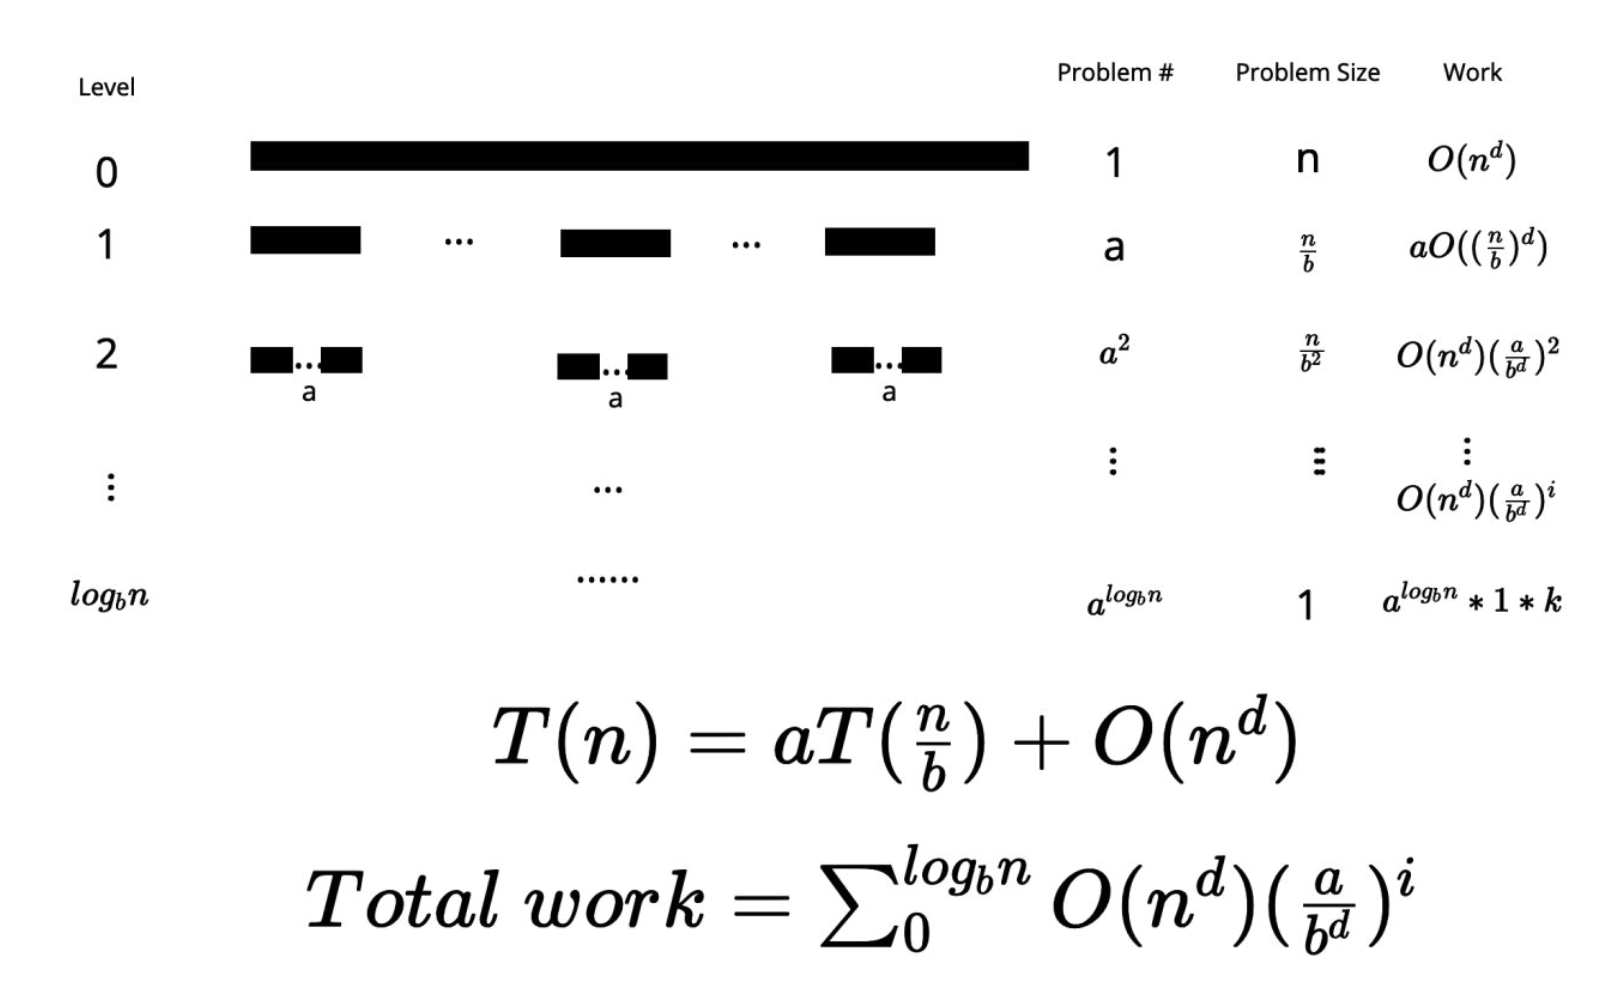
\includegraphics[width=0.8\textwidth]{master-method.png}
\end{figure}
%\begin{figure}[H]
%	\centering
%	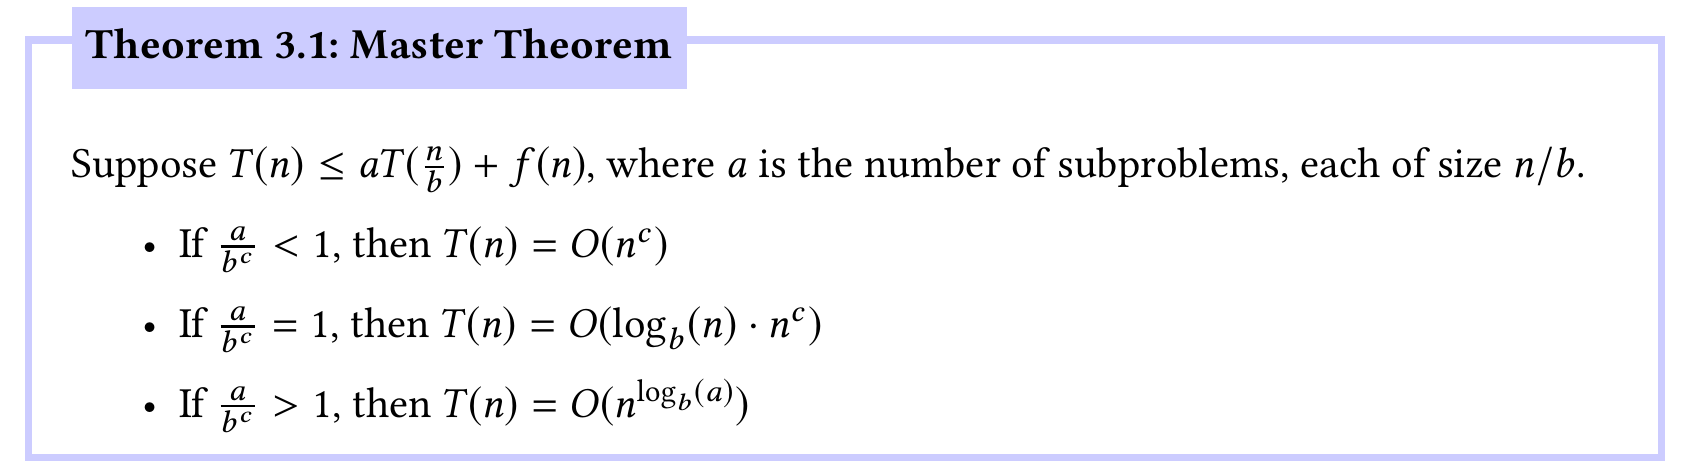
\includegraphics[width=0.5\textwidth]{master-method-2.png}
%\end{figure}
\begin{theorem}
	\textbf{Master Theorem:} Suppose $T(n) \le a T(\frac{n}{b}) + f(n)$, where $a$ is the number of subproblems, each of size $n / b$. Then
	\begin{itemize}
		\item If $\frac{n^c}{n^{\log_b a}} > 1$, the root dominate the running time, then $T(n) = O(n^c)$.
		\item If $\frac{n^c}{n^{\log_b a}} = 1$, intermidiate levels should be considered, then $T(n) = O(log_b n \cdot n^c)$.
		\item If $\frac{n^c}{n^{\log_b a}} < 1$, the leaves dominate the running time, then $T(n) = O(n^{\log_b a})$
	\end{itemize}
\end{theorem}
	
\section{Quick Sort}
\begin{itemize}
	\item Input: Array of $n$ integers.
	\item Outputs: These integers in certain order.
\end{itemize}

\subsection{Algorithm:}
\begin{itemize}
	\item Pick an element $x$ as the pivot element
	\item By comparing each of the elements with the pivot, place it in one
	of the two sets:
	\begin{align*}
	S=\{y:y<x\}\\
	L=\{y:y>x\}
	\end{align*}
	\item Recursively sort $S$ and $L$.
	\item Output $S\times L$.
\end{itemize}

\subsection{Performance:}
\subsubsection{Worst Case}
Each partition routine produces one sub-problem with n-1 elements and one with 
0 elements.
\begin{align*}
T(n)&\ge\Theta(n)+T(n-1)
&\intertext{Based on substitution method,}
T(n)&=\Theta(n^{2})
\end{align*}
\subsubsection{Expected Running Time}
Calculate the expected number of comparison made by QuickSort in the worst 
case when the pivot is selected randomly.
\begin{itemize}
	\item Algorithm: pick pivot uniformly at random from the elements to be
	sorted.
	\item Analysis:
	\begin{itemize}
		\item Let $x$ be the total amount of comparison are formed by QuickSort. 
		\item Let $x_{ij}$ be a random variable that is : 
		
		$$x_{ij}=
		\begin{cases}
		1 & \text{if i-th smallest element and j-th smallest element are compared.}\\
		0 & \text{otherwise.}
		\end{cases}
		$$
		\item $x=\sum_{i<j}x_{ij}$
		\item $E[x]=E[\sum_{i<j}x_{ij}]=\sum_{i<j}E[x_{ij}]$ (Linearity of Expectation)
		$=\sum_{i<j}Pr[x_{ij}=1]$
		\item $x_{i}$ and $x_{j}$ are compared if and only if the first element
		to be chosen as a pivot from $x_{ij}$ is either $x_{i}$ or $x_{j}$.
		\item Pr\{$z_{i}$ is compared to $z_{j}$\} = $\frac{2}{j-i+1}$
	\end{itemize}
	\item 
	Expected 
	Running time
	\begin{align*}
	E[x]&=\sum_{i<j}Pr[x_{ij}=1]
	=\sum_{i<j}\frac{2}{j-i+1}\\
	&=2\sum_{i=1}^{n-1} \sum_{j=i+1}^n \frac{1}{j-i+1}\\
	&=2\sum_{k=1}^{n-1} \frac{n-k}{k+1}\\
	&= 2\sum_{k=1}^{n-1} \frac{n}{k+1} - 2\sum_{k=1}^{n-1}\frac{k}{k+1}\\
	&< 2 \sum_{k=1}^{n-1} \frac{n}{k}\\
	&= O(n\log n)
	\end{align*}
\end{itemize}

\section{Selection/ order}
\begin{itemize}
	\item Input: An array $A$ of n integers and a rank $i$, with $1\ge i\ge n$.
	\item output: The element $x\in A$ that is larger than exactly $i-1$ other
	elements of $A$.
\end{itemize}
We can solve the selection problem in $O(n\log n)$ time since we
can sort the number using heapsort or mergesort and then simply index
the $i$-th element in the output array. But we can do better than this.

\subsection{Randomized-Select}
\begin{algorithm}[H]
	\SetKwProg{Fn}{Function}{:}{}
	\SetKwFunction{FRandSelect}{RANDOMIZED-SELECT}
	\SetKwFunction{FRandPartition}{RANDOMIZED-PARTITION}
	
	\Fn{\FRandSelect ($A, p, r, i$)}{
		%         \KwData{Array $A[p, \cdots, r]$, rank $i$}
		\uIf{p == r}{
			return A[p]
		}
		q = \FRandPartition(A, p, r){}
		
		k = q - p + 1 
		
		\uIf {i == k}{\tcc{The pivot is the answer}
			return A[q]
		}
		\uElseIf {i < k}{
			return \FRandSelect ($A, p, q-1, i$)
		}
		\Else{
			return \FRandSelect ($A, q+1, r, i-k$)
		}
		
	}
	\caption{Randomized-Select}
\end{algorithm}
The worst-case running time for RANDOMIZED-SELECT is $\Theta(n^2)$, because we 
could be extremely unlucky and always partition around the largest remaining 
element, and the partition takes $\Theta(n)$ times.

But the algorithm has a linear expected running time $O(n)$, and because it is 
randomized, no particular input elicits the worst-case behavior.

\subsection{Deterministic Linear Time Selection}
After quick selection, algorists looked for an algorithm which is able to solve 
the problem in linear deterministic.

\centerline{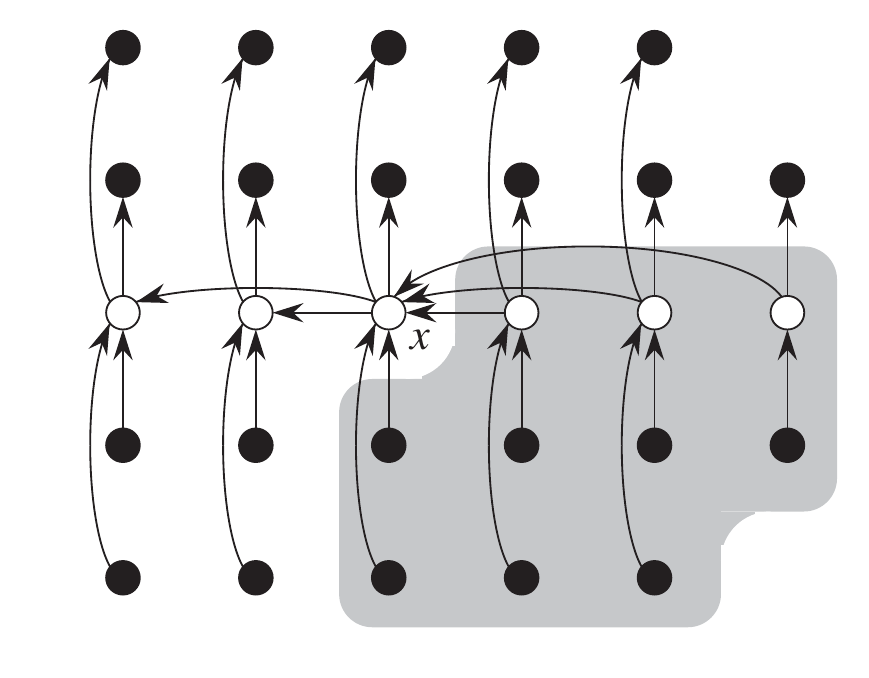
\includegraphics[width=0.5\textwidth]{deterministic-select.png}}
Given an array with $n$ numbers, we can find the element with rank $i$ by the following method.
	
SELECT Algorithm:
\begin{itemize}
	\item Partition the numbers into groups of size 5.
	\item Find the medium of each group. It can be done within 6 comparisons. $T(n) = \frac{6n}{5} 
	= 1.2n$.
	\item Use SELECT to recursively find the medium of the mediums $m^*$.
	\item $m^*$ has a rank somewhere in the middle.
	We treat the median of the medians $m^*$ as a pivot element and compare it with all elements to get its rank $k$, which takes $n$ steps.
	\begin{itemize}
		\item The number of elements larger than $m^*$: $O(\frac{3n}{10}) 
		=3(\ceil*{\frac{1}{2}\ceil*{\frac{n}{5}}})$
		\item Therefore, the number of element smaller than $m^*$: 
		$O(\frac{7n}{10})$.
	\end{itemize}
	\item Pivot using $m^*$:
	\begin{itemize}
		\item If $i = k$, then return $k$.
		\item If $i < k$, use SELECT recursively to find the $i$-th smallest 
		element on the low side.
		\item If $i > k$, use SELECT recursively to find the $(i-k)$-th smallest 
		element on the high side.
	\end{itemize}
\end{itemize}
Therefore, the recursion of the algorithm is
\[T(n) \le T(\frac{n}{5}) + T(\frac{7n}{10}) + 2.2n\]
The expression does not fit into the master theorem frame work because of the 
two different size of the sub-problems. Then we guess $T(n) \le 22n$ and it can 
be proved by induction.
\begin{itemize}
	\item Base case:
	
	Base case it trivial and we skip it during the class because 22 is a 
	fairly large number. It should be easy find a number $n$ so that we could 
	calculate $T(n)$ easily and show that it is less than $22n$.
	
	\item Hypothesis: Suppose each of the cost satisfies $T(n) \le 22n$ for $(0, 
	n)$. 
	
	Therefore, 
	\begin{align*}
	T(\frac{n}{5}) &\le 22 \times \frac{n}{5}\\
	T(\frac{7n}{10}) &\le 22 \times \frac{7n}{10}\\
	\intertext{so that}
	T(n) &\le 22 \times 0.2 n + 22 \times 0.7 n + 2.2n
	\end{align*}
	\item Inductive step:
	\begin{align*}
	T(n) &\le 22 \times 0.2 n + 22 \times 0.7 n + 2.2n\\
	T(n) &\le 22 \times (0.2 + 0.7 + 0.1)n\\
	T(n) &\le 22n
	\end{align*}
\end{itemize}

\subsection{Efficiently Find Median in a Small Gorup}
The following algorithm gives pretty good upper bounds for finding the median for a small number of elements, although they are not the best upper bounds
for n > 6.

Suppose we are trying to find the $t$-th largest element of n,
\begin{itemize}
	
	\item Choose $n - t + 2$ of the elements arbitrarily, and find the largest one by tennis tournament like procedure. 
	
	\item Replace the largest element by one of the elements that hasn't yet participated in the tournament and make it play the same opponents that the largest element played to determine the new largest. r
	
	\item We keep doing this until all the elements that were set aside initially have played in the tournament. 
	
	\item We replace the largest element of the last round too (and hence are left with n - t + 1 elements).
	
	\item Now the largest element that remains is the one we are looking for.
\end{itemize}

\subsubsection{Correctness}
There are at most $(t-2)$ numbers larger than the largest element in the $(n - t + 2)$ element, say $x$. Every $x$ is the one of the top $t-1$ numbers. We repeat the tournament $t-1$ times to find all the top $t-1$ numbers. Then the largest one in the rest of $n - t + 1$ numbers has the rank $t$.

\subsubsection{Time}
\begin{itemize}
	\item The first tournament takes $(n - t + 1)$ comparisons. 
	\item Then the next $t - 2$ tournament only take $\log_2 (n - t + 2)$ times. \item Finally, find the one with rank $t$ takes one more tournament among $(\log_2 n - t + 2)$ elements.
\end{itemize}

\[T(n) = (n - t + 1) + (t -2 )\log_2 (n - t + 2) + \log_2 (n - t + 2)\]




\section{Polynomial Multiplication}
\subsection{Introduction}
A polynomial in the variable x over an algebraic field $F$ represents a function 
$A(x)$ as a formal sum:
\[A(x) = \sum_{j = 0}^{n-1} a_j x^j\]
We call the values $a_0, ~a_1, ~\cdots, ~a_{n-1}$ the \textbf{coefficients} of 
the polynomial. The coefficients are drawn from a field $F$ , typically the set 
$\mathbb{C}$ of complex numbers. A polynomial can be represented as a list of 
coefficients in computer.

A polynomial $A(x)$ has \textbf{degree $k$} if its highest nonzero coefficient 
is $a_k$. We write that $\text{degree}(A) = k$. Any integer strictly greater 
than the degree of a polynomial is a \textbf{degree-bound }of that polynomial. 
Therefore, the degree of a polynomial of degree-bound $n$ may be any integer 
between $0$ and $n-1$, inclusive.

Polynomial Multiplication: if $A(x)$ and $B(x)$ are polynomials of degree-bound 
$n$, their product $C(x)$ is a polynomial of degree-bound $2n - 1$ such that
$C(x) = A(x)B(x)$ for all $x$ in the underlying field. For example,

\centerline{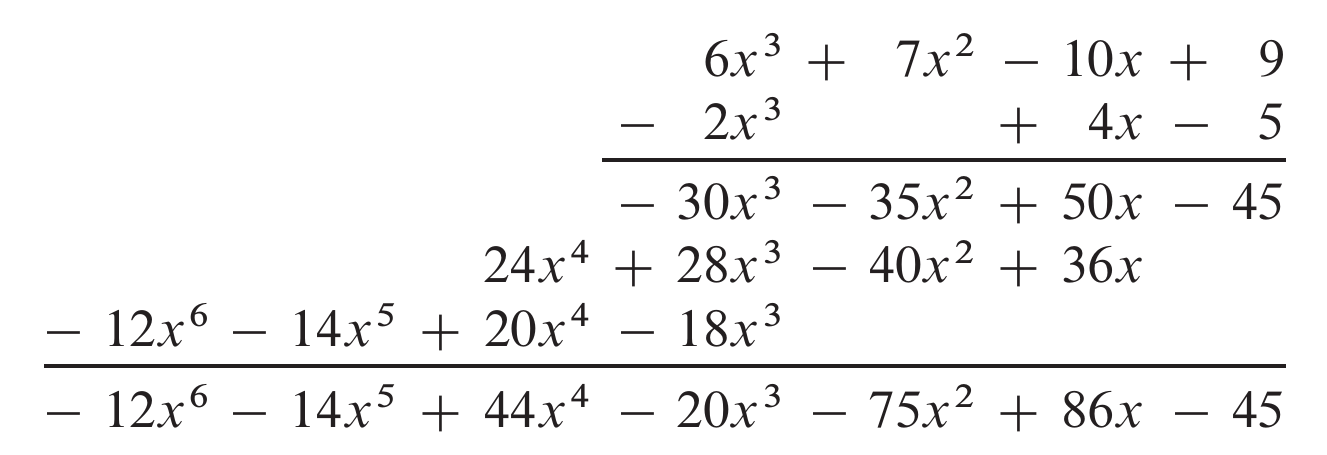
\includegraphics[width=0.5\textwidth]{poly-multiply.png}}

Another way to express the product $C(x)$ is
\begin{align*}
 C(x) = \sum_{j=0}^{2n-2} c_j x^j\\
 \intertext{where}
 c_j = \sum_{k=0}^j a_k b^{j-k}
\end{align*}

Note that $\text{degree}(C) = \text{degree}(A) +  \text{degree}(B)$, implying 
that if $A$ is a polynomial of degree-bound $n_a$ and $B$ is a polynomial 
of degree-bound $n_b$ , then $C$ is a polynomial of degree-bound $n_a + n_b - 
1$. Since a polynomial of degree-bound $k$ is also a polynomial of degree-bound 
$k + 1$, we will normally say that the product polynomial $C$ is a polynomial 
of degree-bound $n_a + n_b$.

\subsection{Algorithm}
Input: Two polynomials with same degree $d$:
\begin{align*}
 A &= a_d x^d + \cdots + a_0\\
 B &= b_d x^d + \cdots + b_0
\end{align*}
Goal: Calculate the product of the inputs.

\subsubsection{Baseline Method}
Simply calculate each parameter based on the definition of polynomial product. 
Each parameter in $A(x)$ should multiply all the parameters in $B(x)$ 
which takes $O(n^2)$ steps.
\subsubsection{Divide and Conquer}
\textbf{Assumption}: To make sure the parameters could be nicely divided by 
two, we assume the degree $d$ of both polynomials is always $2^k - 1$, where $k 
\in \mathbb{N}$.

Divide the $(d+1)$ entries of polynomials as follows to reduce the problem size:

\centerline{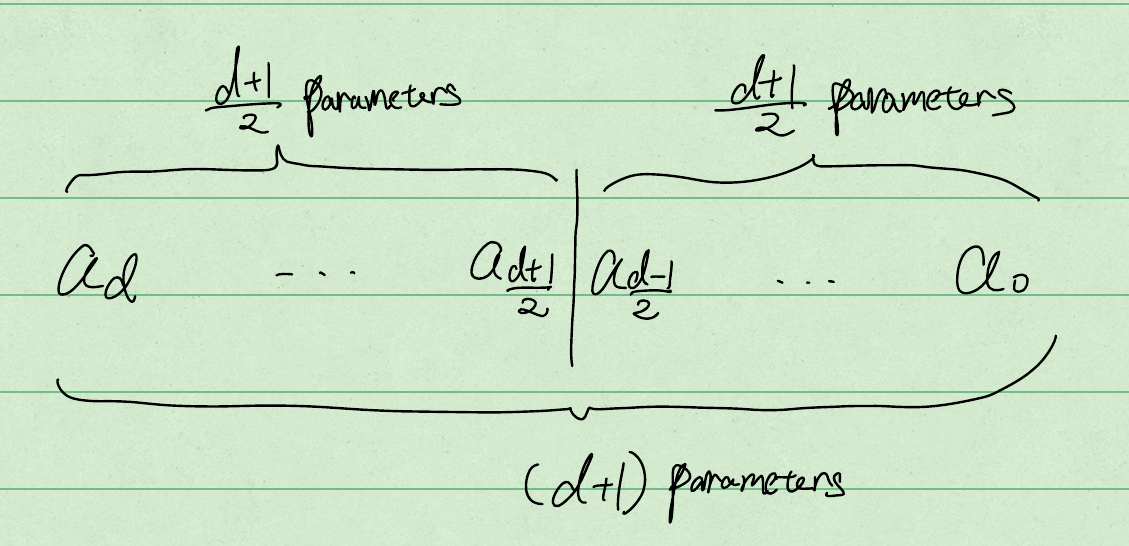
\includegraphics[width=0.5\textwidth]{poly-devide.png}}

Call the right hand side of polynomial as $A_l$. Extract $x^{\frac{d+1}{2}}$ 
and call the left hand side of polynomial as $x^{\frac{d+1}{2}} A_h$. we have,
\begin{align*}
 A &= x^{\frac{d+1}{2}} A_h + A_l\\
 B &= x^{\frac{d+1}{2}} B_h + B_l\\
 \intertext{Based on the algebra,}
 A \times B &= (x^{\frac{d+1}{2}} A_h + A_l)(x^{\frac{d+1}{2}} B_h + B_l)\\
 &= x^{d+1}A_h B_h + x^{\frac{d+1}{2}}A_h B_l + x^{\frac{d+1}{2}}A_l B_h + A_l 
B_l
\end{align*}
Therefore, we reduce the problem into four sub-problems with half of the size. 
Suppose the number of parameters is $n$, i.e. the degree of polynomials is $d = 
n - 1$. The recursion equation as follows:
\[T(n) \le 4T(\frac{n}{2}) + cn\]
Based on master theorem, $T(n) = O(n^2)$. Unfortunately, we have not get any 
improvement from those nicely splits comparing with the baseline. If you think 
about it, the result is actually not surprising because even though the problem 
size is reduced, we could not skip any of the necessary multiplication. In 
other words, there are still $n^2$ necessary multiplications to get the 
production.

\textbf{Motivation}: When you have a recursive algorithm, saving  one operation 
could have a cascade effect and reduce the run time quickly. Adding polynomials 
only costs $O(n)$ steps. If we could reduce multiplications by introducing 
addition. Then we are able to achieve better performance. 

To reduce the multiplications by adding additions, we have
\begin{align*}
 A \times B &= x^{d+1}A_h B_h + x^{\frac{d+1}{2}}A_h B_l + x^{\frac{d+1}{2}}A_l 
B_h + A_lB_l\\
            &= x^{d+1}A_h B_h + x^{\frac{d+1}{2}}(A_h B_l + A_l B_h) + A_l 
B_l
\end{align*}
Therefore, there are three items to calculate
\begin{enumerate}[(1)]
 \item $A_h B_h$
 \item $A_l B_l$
 \item $A_h B_l + A_l B_h$
\end{enumerate}
(1) and (2) are two multiplications. Moreover, (3) can be calculate by one more 
multiplication as following:
\begin{align*}
 &  (A_h + A_l) (B_h + B_l) - A_h B_h - A_l B_l\\
 =& A_hB_h + A_hB_l + A_lB_h + A_lB_l - A_h B_h - A_l B_l\\
 =& A_lB_h + A_hB_l
\end{align*}

Therefore, the recursive function becomes
\[T(n) \le 3T(\frac{n}{2}) + cn\]
It can be solved by master theorem, where $a = 3, b = 2, c = 1$.

Since $\log_ba > 1 = c$, so $T(n) = O(n^{\log_2 3}) \approx O(n^{1.6})$

\section{Convex Hull on the Plane}
\subsection{Introduction}
\subsubsection{Convex set}
Convex set A set $S \subseteq \mathbb{R}^n$ is said to be convex if $\forall 
x,y \in S$, the line segment joining $x$ and $y$ is contained in $S$.

\centerline{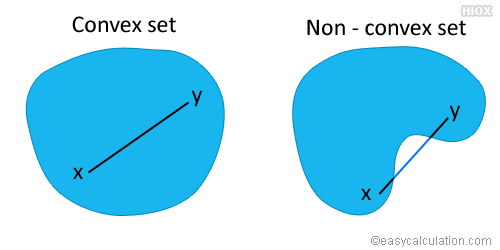
\includegraphics[width=0.5\textwidth]{convex-nonconvex-set.png}}
\subsubsection{Convex Combination}
Given two points $x=(x_1, x_2)$ and $y = (y_1, y_2) \in \mathbb{R}^2$, a convex 
combination of $x$ and $y$ is defined by
\[\lambda x + (1 - \lambda) y = \lambda x_1 + (1 - \lambda)y_1 + \lambda x_2 + 
(1 - \lambda)y_2, \text{ for } \lambda \in [0,1]\]
Changing the value of $\lambda$, we walk thought the segment. In general, 
 is the area confined by the edges formed by points.
 
 \paragraph{Example} Consider a practical example, suppose there are four wells 
$(w_1, w_2, w_3, w_4)$ to generate petroleum and the composition $(A, B, C)$ of 
petroleum from each well are different as follows:

\begin{table}[H]
\centering
\begin{tabular}{|l|l|l|l|l|}
\hline
            &       & A   & B   & C   \\ \hline
$\lambda_1$ & $w_1$ & 0.4 & 0.4 & 0.2 \\ \hline
$\lambda_2$ & $w_2$ & 0.6 & 0.3 & 0.1 \\ \hline
$\lambda_3$ & $w_3$ & 0.3 & 0.4 & 0.3 \\ \hline
$\lambda_4$ & $w_4$ & 0.2 & 0.7 & 0.1 \\ \hline
\end{tabular}
\end{table}
Therefore, all the possible compositions from the mixture of the four kinds of 
petroleum is actually a convex combination of the four petroleum. The four 
wells are like four points in a 3-D space and the convex set is the object 
whose vertices are those four points.

\subsubsection{Convex Hull}
\textbf{Definition 1}: Convex hull of a finite set of points $S$ is the set of 
all points that can be expressed as convex combinations of points in $S$. 

\textbf{Definition 2}: Convex hull of a set of points is the smallest convex 
set that contains these points.
 
More intuitively, convex hull is like a rubber band stretched from infinite and 
struck on the nails on points.
\centerline{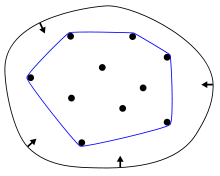
\includegraphics[width=0.5\textwidth]{ConvexHull.png}}
\subsubsection{Convex polygon}
Convex polygon is a polygon which is a convex set. It always contains interior 
angle which smaller than 180 degree.
\subsection{Algorithm}
\begin{itemize}
 \item Input: $n$ points, $(x_1, y_1), (x_2, y_2), \cdots, (x_n, y_n)$.
 \item Output: The sequence of points on the boundary in counter clock order.
\end{itemize}

\subsubsection{Relative Location of Line and Points}
Given a line by two points $(x_1, y_1), (x_2, y_2)$ , a joining segment can 
be represented as follows:
\[y - y_1 = \frac{y_1 - y_2}{x_1 - x_2} (x - x_1)\]

For any third point $(x_3, y_3)$, it is possible determine which side of the 
line the third point lies. For instance, the thirds point is above the segment 
if 
\[y_3 - y_1 > \frac{y_1 - y_2}{x_1 - x_2} (x_3 - x_1)\]

\subsubsection{Convex Hull Successive Points Lemma}
\begin{itemize}
 \item If there is a segment joining two points such that all the other 
points lie on the same side of the segment, the segment represents two points 
on the convex hull.
 \item Conversely, if you have a segment on the convex hull and extending it, 
then every point from the convex hull will lie on the same side of the line.
\end{itemize}

\subsubsection{Baseline}
\begin{enumerate}
\item Use the extreme point as a start $x$.
\item Take every pair of points with $x$. write the equation for the line 
joining them and find the line where all other the points lie on the same side.
\item The line is a segment of convex hull.
\item Set $x$ to the other point of the segment and then repeat step 2.
\end{enumerate}

\paragraph{Runing Time Analysis}
\begin{itemize}
\item Determine all the points are on the same side of segment takes $O(n)$ 
steps.
\item To find one convex hull segment, we should check $O(n)$ segments.
\item There are at most $O(n)$ convex hull segment.
\item Therefore, the total run time is $O(n^3)$.
\end{itemize}

\subsubsection{Merge Hull}
Tips: To be efficient, we could like the sizes of sub-problems in divide and 
conquer to be same.
\begin{enumerate}
 \item Divide points into those with $x$-coordinates $\le x_{median}$ and those 
with $x$-coordinates $> x_{mdian}$.
\item Recursively find the convex hull for the points on the left and right.
\item Find the upper tangent and lower tangent of the two convex hull. 
\item Start from the left of upper tangent and walk through the left convex 
hull counterclockwise until meet the lower tangent. Then move to the right 
convex hull and keep walking until back to the upper tangent.
\end{enumerate}
\centerline{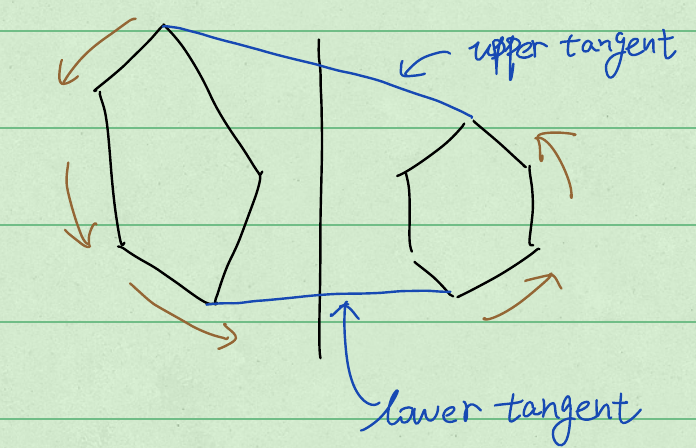
\includegraphics[width=0.5\textwidth]{tangent.png}}

\paragraph{Remarks:}
\begin{itemize}
\item Points on one hull can ``\textbf{see}'' a point on the other hull if the 
segment joining the two points does not intersect either hull.
\item Upper tangent, lower tangent are pairs of points that see each other.
\item \textbf{Upper tangent}  is the highest line segment joining two vertices, 
one from each hull, that see each other.
\item Similar with the lower tangent. Therefore the total running time is 
$O(n)$.
\end{itemize}

\paragraph{Stab}
A line $pq$ stabs to $C_2$ if the continuation of the line goes to 
the interior of $C_2$.

\paragraph{How to check stabbing}
\begin{itemize}
\item If the segment $pq$ stabs $C_2$, then the clockwise predecessor of $q$ 
is on the one side of the segment and the clockwise successor of $q$ is one the 
other side.
\item If $pq$ stabs $C_2$ then $p$ must be able to see the clockwise 
predecessor and successor of $q$.
\end{itemize}

\paragraph{How to find the upper tangent:}
The upper tangent can be found by a ``swirling'' algorithm.
\begin{itemize}
\item Choose $p$ to be the right most point in the left hull ($C_1$) and 
$q$ to be the left most point in the right hull ($C_2$). Then $p$ and $q$ see 
each other. 
\item If $pq$ stabs to $C_1$, move $p$ to its counterclockwise successor.
\item If $pq$ stabs to $C_2$, move $q$ to its clockwise successor.
\item repeat until $pq$ does not stab to any hull. Then $pq$ is the upper 
tangent.
\end{itemize}

Lower tangent can be find with the similar strategy.

\paragraph{Running Time Analysis}
We never repeat the same pair of vertices since once you decide to abandoned a 
vertex in searching of upper tangent, you never come back to it. It means at 
most $n$ vertices to find the upper tangent.

Similarly for the lower tanget.

\subsubsection{Quick Hull}
Like QuickSort, Quick Hull does not have worst case analysis.
\begin{itemize}
\item Pick the left most point $p$ and right most point $q$ on the convex hull 
and draw a segment joining them.
\item Recursively find the convex hull for each side of the points. Each hull 
must contains the segment $pq$.
\item Merge the two hull by glue them on segmeng $pq$.
\end{itemize}

We did not spend too much time on how to find the next two pair of points at 
each iteration. But here are some remarks.

\paragraph{Remarks}
\begin{itemize}
 \item Always pick points on $x$ direction my casue the worst case, which is 
all the points are aggregated to one side of line.
\item Like quicksort, introducing randomness helps achieve the optimal average 
running time. We randomly choose a direction and project all the points on it. 
Pick the two extremes as the points for the next iteration.
\end{itemize}

\end{document}
